% !TEX root = www2019-visual-ltr.tex


\begin{figure}[t]
\begin{tabular}{ccc}
\subfloat{
\includegraphics[width = 1in]{images/1-snapshot.png}} &
\subfloat{
\includegraphics[width = 1in]{images/1-highlights.png}} &
\subfloat{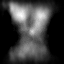
\includegraphics[width = 1in]{images/1-saliency.png}} \\
\subfloat{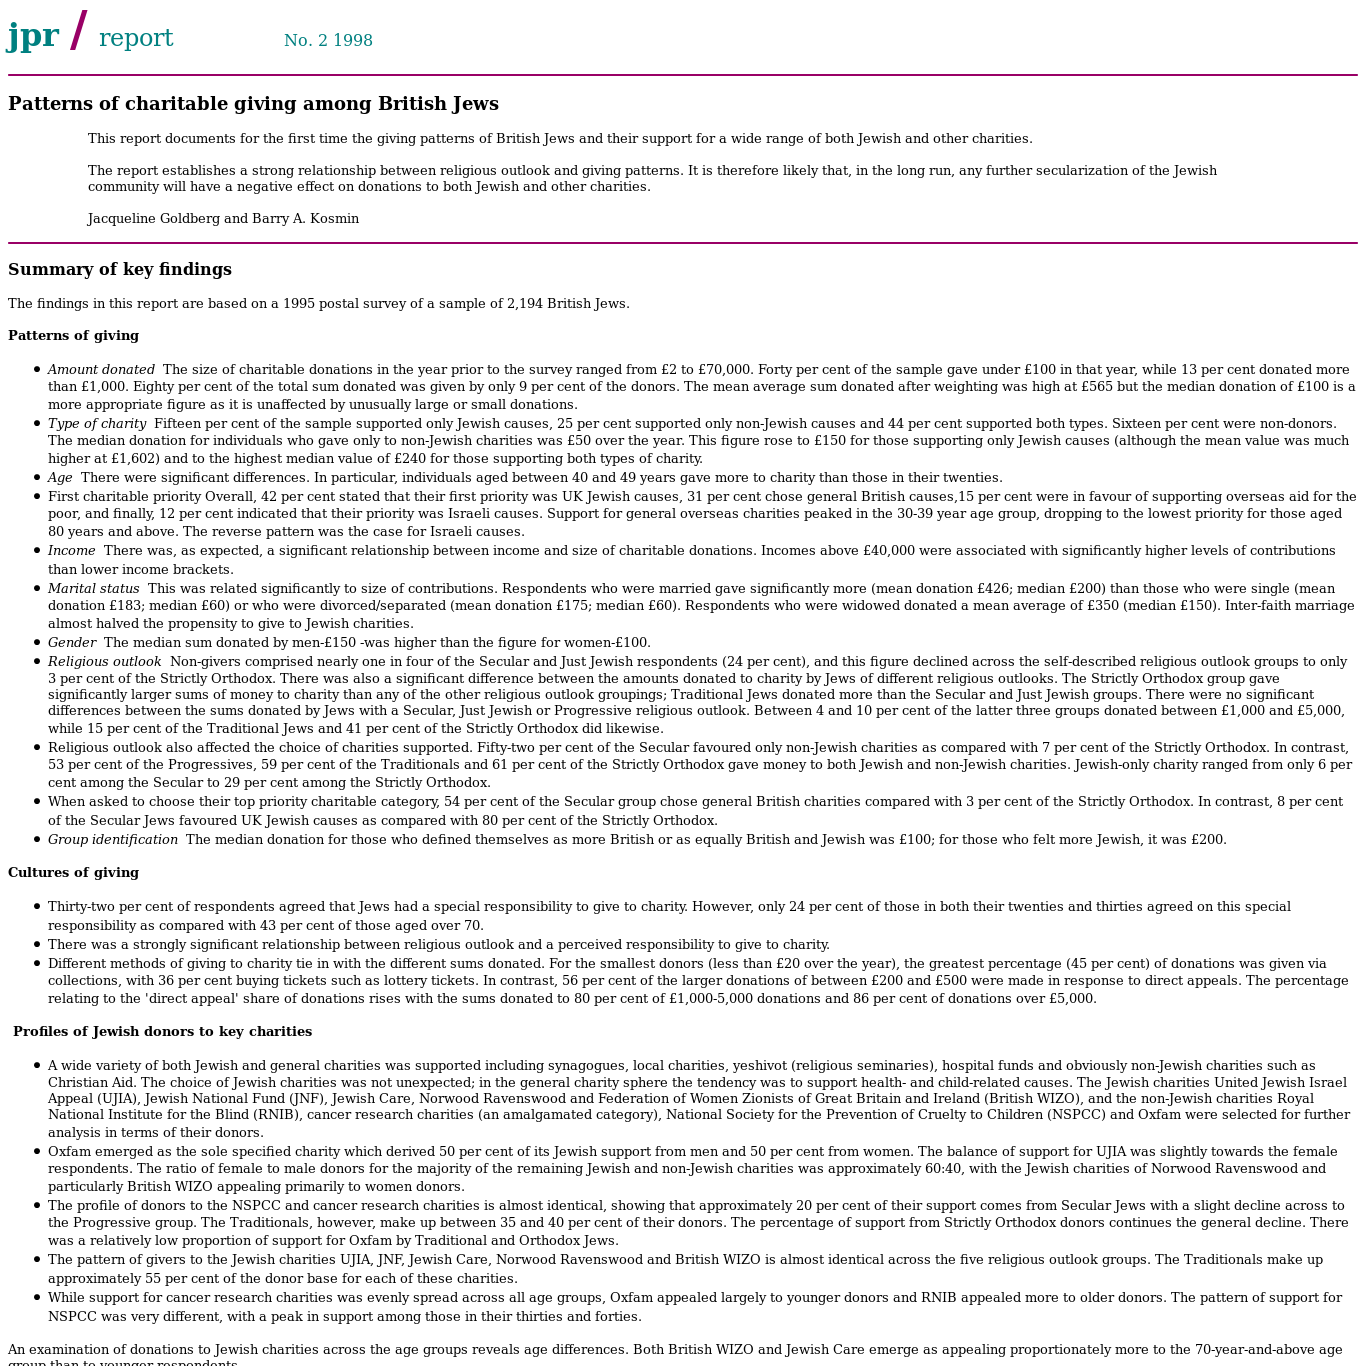
\includegraphics[width = 1in]{images/2-snapshot.png}} &
\subfloat{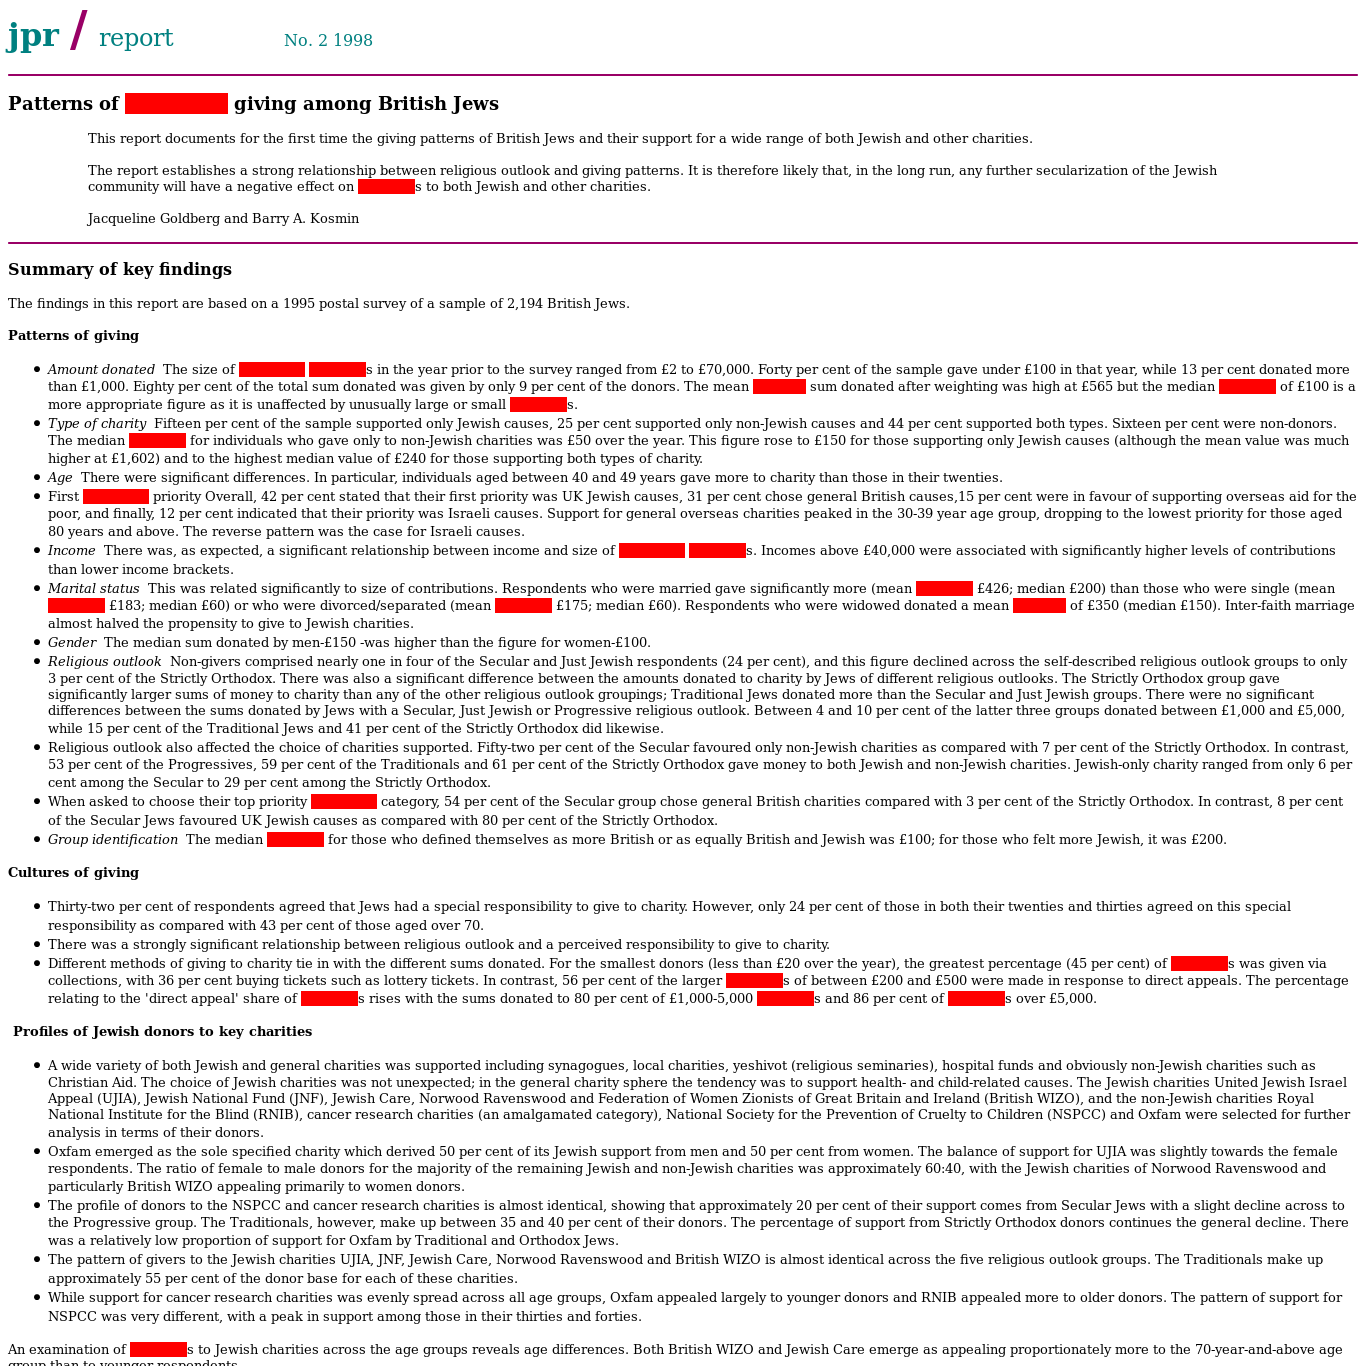
\includegraphics[width = 1in]{images/2-highlights.png}} &
\subfloat{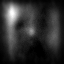
\includegraphics[width = 1in]{images/2-saliency.png}} \\
\subfloat{
\includegraphics[width = 1in]{images/3-snapshot.png}} &
\subfloat{
\includegraphics[width = 1in]{images/3-highlights.png}} &
\subfloat{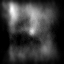
\includegraphics[width = 1in]{images/3-saliency.png}} \\
\end{tabular}
\caption{Examples of a vanilla snapshot, a red highlighted snapshot, and a saliency heatmap from left to right, respectively.}
\label{fig:exampleshots}
\end{figure}


\section{\protect\datasetname{} Data\-set}
In this section, we introduce the \datasetname~data\-set for \ac{LTR} with visual features. 
Section~\ref{sec:trecclue} contains information about the underlying ClueWeb12 collection and TREC Web Track topics.
Section~\ref{sec:screenshotsec} explains how the snapshots for ClueWeb12 are acquired.
% using the Wayback Machine\footnote{\url{http://archive.org/web/}} and ClueWeb12 Online rendering service.\footnote{\url{http://boston.lti.cs.cmu.edu/Services/}}
Section~\ref{sec:contentfeature} discusses content features, such as BM25 and TF-IDF, included in the \datasetname{} dataset.
Finally, Section~\ref{sec:finalcollection} gives an overview of the structure in which the \datasetname~dataset is presented and published.

\subsection{ClueWeb12 \& TREC Web Track}\label{sec:trecclue}
For the \datasetname{} dataset we choose to use a combination of the ClueWeb12 document collection and the topics from the TREC Web Tracks 2013 \& 2014~\cite{collins2013trec,collins2015trec},
because this is currently the most recent combination of a large-scale webpage collection together with judged queries (with graded relevance). 

ClueWeb12 is a highly diverse collection of webpages scraped in the first half of 2012.
The total collection contains over 700 million webpages.
%that are crawled using the typical crawling settings of the Heritrix archival crawler project.\footnote{\url{https://webarchive.jira.com/wiki/spaces/Heritrix/overview}}
%
We only use ClueWeb12 webpages that have judgements for any of the 100 queries in the TREC Web Tracks 2013 \& 2014.
In total, there are 28,906 judged webpages.
%
Table~\ref{tab:countsources} shows the breakdown of the total number of webpages and different relevance labels in the combined set of topics from 2013 and 2014.

\begin{table}[h]
  \captionof{table}{Number of webpages per source and the corresponding breakdown of TREC Web Track relevance grades.} 
  \label{tab:countsources}
  \begin{tabular}{ l  @{}r  r  r  r }
  \toprule
    Count/Label & TREC Web & Wayback & ClueWeb12 & \mbox{}\hspace*{-.15cm}No image\\
    \midrule
    Total & 28,906 & 23,249 & 5,392 & 265 \\
    Nav grade (4) & 40 & 36 & 4 & 0\\
    Key grade (3) & 409 & 347 & 62 & 0\\
    Hrel grade (2) & 2,534 & 2,222 & 295 & 17 \\
    Rel grade (1) & 6,832 & 5,679 & 1,123 & 30\\
    Non grade (0) & 18,301 & 14,395 & 3,701 & 205 \\
    Junk grade (-2) & 790 & 570 & 207 & 13\\
    \bottomrule
  \end{tabular} 
\end{table}


\subsection{Snapshots} \label{sec:screenshotsec}
Although each entry in the ClueWeb12 collection contains the webpage's HTML source, many pages lack styling and images files in order to render the full page.
To overcome this issue, we use the Wayback Machine,\footnote{\url{http://archive.org/web/}} which offers various archived versions of webpages with styling and images since 2005.
For each page in ClueWeb12, that is also judged in the TREC Web Tracks 2013 \& 2014,
we scrape an entry on the Wayback Machine that is closest to the original page scrape date as recorded in ClueWeb12.
A snapshot is then taken using a headless instance of the Firefox browser.
%together with the Python implementation of the Selenium testing framework.\footnote{\url{http://selenium-python.readthedocs.io/}}
To reproduce \cite{fan2017learning}, we also create a separate query-dependent dataset with the same snapshots where all query words are highlighted in red (HEX value: \#ff0000).
Examples of snapshots and snapshots with highlights are shown in Figure~\ref{fig:exampleshots} (first two columns). 


\label{sec:datasetsum}
Since the Wayback Machine does not contain an archived or working version of each webpage in the ClueWeb12 collection, a filtering process is introduced to maximize the quality of each snapshot. Using the following criteria, a snapshot is selected for each available webpage. 
\begin{enumerate}[leftmargin=14pt]
\item Each webpage is requested from the Wayback Machine. 
\item A webpage that is not on the Wayback Machine, times out, throws a JavaScript error, or results in a PNG snapshot smaller than 100KB is marked as broken. Such webpages are rendered again using the online rendering service provided by ClueWeb12.\footnote{\url{http://boston.lti.cs.cmu.edu/Services/}}
\item A manual selection is made between all webpages that are rendered from both sources. The Wayback version is used if it contains more styling elements and if the content is the same as in the rendering service. Otherwise, the rendering service version is used. 
\end{enumerate}
%
As a result, most of the 28,906 judged webpages have a corresponding snapshot from either the Wayback Machine or ClueWeb12 rendering service.
Only 265 documents did not pass the filtering and were discarded.
Table~\ref{tab:countsources}, row one, summarizes the results of the \datasetname{} dataset~acquisition process. Additionally, the table also shows the distribution of judgment scores among the snapshots that were taken from the Wayback Machine and ClueWeb12 rendering service.


\subsection{Non-Visual Features} 
\label{sec:contentfeature}
In LTR, documents are ranked based on various types of features, such as content features (e.g., BM25), quality indicators (e.g., PageRank) and behavioral features (e.g., CTR).
In order to use the \datasetname{} dataset to measure the effect of visual features, we also add a set of content features and quality indicators,
listed in Table~\ref{tab:setdescription}.
These 11 features are chosen so that they resemble most informative features of the most recent LETOR 4.0 dataset~\cite{Qin2013:Introducing} and are easy to compute
(see Section~\ref{sec:contentfeatures} for a detailed comparison of different feature sets).
%We further elaborate on this and compare different feature sets in Section~\ref{sec:discussion}.
Also note that behavioral features, such as CTR, are not available for the TREC Web Tracks.

\if0
The content features are computed by doing a full pass over the complete ClueWeb12 collection using Apache Spark.\footnote{\url{https://spark.apache.org/}}$^{ }$\footnote{This took approximately 20 hours on 116 Hadoop worker nodes with 3 executor cores and 21Gb memory each.}
During this process an HTML parser (jsoup\footnote{\url{https://jsoup.org/}}) extracts the title and content from the raw HTML.
Because the HTML structure in very large documents cannot be parsed efficiently by jsoup, all documents with more than one million tokens are ignored.
Using the Apache Spark implementation of TF and IDF, a sparse vector is obtained for each term in each document. Finally, the sparse vectors are loaded into a Python Pandas dataframe, which is used to compute the TF, IDF, TF-IDF and BM25 scores for each document-query pair.
\fi

The content features, such as TF-IDF and BM25, are computed by doing a full pass over the complete ClueWeb12 collection.
The PageRank scores are taken from the ClueWeb12 Related Data section.\footnote{\url{https://lemurproject.org/clueweb12/related-data.php}}
The following modifications based on the feature transformations described in LETOR are made to stabilize training:
\begin{enumerate}[leftmargin=14pt]
% \item IDF is calculates as follows: 
% $$IDF(q, D) = \sum_{t_i \in q} IDF(t_i, D) = \sum_{t_i \in t} \log \frac{|D| + 1}{DF(t_i) + 1}$$
% Where  $q_i$ and $t_i$ represent a list of all terms in a query and a single query term respectively. $D$ represents a list of all terms in a document with $|D|$ as its total length. $DF(t_i)$ is the document frequency for the given query term.  
\item Free parameters $k_1$, $k_3$ and $b$ for BM25 were set to $2.5$, $0$ and $0.8$, respectively. 
\item Since the PageRank scores are usually an order of magnitude smaller than all other scores, we multiply them by $10^5$.
\item The log transformation is applied to each feature.
\item The log-transformed features are normalized per query.  
\end{enumerate}

\begin{table}[h]
\centering
\captionof{table}{Non-visual features provided with the \datasetname{} dataset.}  \label{tab:setdescription} 
\begin{tabular}{rlrlrl}
\toprule
Id & Description & Id & Description & Id & Description    \\ 
\midrule
1  & Pagerank  & 5  & Content TF-IDF  & 9  & Title IDF   \\
2  & Content length & 6  & Content BM25   & 10 & Title TF-IDF   \\
3  & Content TF  & 7  & Title length & 11 & Title BM25  \\
4  & Content IDF & 8  & Title TF  & & \\
\bottomrule
\end{tabular}
\end{table}

\subsection{Final Collection}\label{sec:finalcollection}
In summary, the \datasetname{} dataset contains:
\begin{inparaenum}[(i)]
\item a directory with webpage snapshots (Section~\ref{sec:screenshotsec}), and
\item a set of files with content features divided into folds (Section~\ref{sec:contentfeature}).
\end{inparaenum}
Each snapshot is stored as a PNG file that can be identified by its corresponding ClueWeb12 document id. 
The non-visual features are stored in LETOR formatted files containing the raw, logged and query normalized values.
The query normalized values are randomly split per query into five equal partitions.
These partitions are then used to create five folds, where each fold contains three partitions for training and the remaining two partitions for validation and testing.
%The \datasetname{} dataset is available at \url{http://anonymized.url}.


%A separate file contains an entry for each snapshot indicating whether the snapshots was created using the Wayback Machine or online rendering service. 

